%@TheDoctorRAB
%standard white paper/preproposal format
%
%%%%%
%
%REFERENCES
%
%neup.bst - numbered citations in order of appearance, short author list with et al in reference section
%nsf.bst - numbered citations in order of appearance, full author list in references section
%standard.bst - citations with author last name with et al for more than 2 authors; full author list in references section
%ans.bst is for ANS only. 
%
%author = {Lastname, Firstname and Lastname, Firstname and Lastname, Firstname} for all bst formats
%bst renders the author list itself
%
%author = {{Nuclear Regulatory Commission}} if the author is an organization, institution, etc., and not people
%
%title = {{}} for all
%
%for all - use \citep{-} - [1] or (Borrelli, 2021) in the text
%standard.bst \cite{-} - Borrelli (2021) in the text
%standard.bst lists references alphabetically
%the rest list numerically
%
%
%%% slides 
%
%\citep{xxxnna} where the citation should go
%\blfootnote{\fontsize\cite{xxxnna}\fontsize\bibentry{xxxnna}} before \end{frame}
%
%
%%%%%

%%%%% presentation settings
\documentclass[aspectratio=1610,pdftex,dvipsnames,compress,xcolor={dvipsnames}]{beamer}
\usetheme{Boadilla}
\usecolortheme{seahorse}
\beamertemplatenavigationsymbolsempty
\addtobeamertemplate{footnote}{\hskip -2em}{} %pushes footnote to margin
\setbeamerfont{title}{series=\bfseries}
\setbeamertemplate{page number in head/foot}[framenumber] %just gives slide number; comment out for 1/7, 2/7...
\definecolor{BackGround}{RGB}{255,250,240}
\setbeamercolor{background canvas}{bg=BackGround}
%%%%%


%%%%% general 
%\documentclass[11pt,a4paper]{article}
%\usepackage[lmargin=1in,rmargin=1in,tmargin=1in,bmargin=1in]{geometry}
\usepackage[pagewise]{lineno} %line numbering
\usepackage{setspace}
\usepackage{ulem} %strikethrough - do not \sout{\cite{}}
\usepackage{graphicx}
\usepackage{mypythonhighlight,verbatim}
\usepackage{filecontents}
\usepackage{tablefootnote}
\usepackage{footnotehyper}
\usepackage{float}
%\usepackage{subfig}
\usepackage[yyyymmdd]{datetime} %date format
\renewcommand{\dateseparator}{.}
\graphicspath{{img/}} %path to graphics
\setcounter{secnumdepth}{5} %set subsection to nth level
\usepackage{needspace}
\usepackage[stable,hang,flushmargin]{footmisc} %footnotes in section titles and no indent; standard.bst
\usepackage[inline]{enumitem}
\setlist[itemize]{label=\textbullet}
\usepackage{boldline}
\usepackage{makecell}
\usepackage{booktabs}
\usepackage{amssymb}
\usepackage{gensymb}
\usepackage{amsmath,nicefrac}
\usepackage{physics}
\usepackage{lscape}
\usepackage{array}
\usepackage{chngcntr}
\usepackage{hyperref}
\hypersetup{colorlinks,linkcolor=black,citecolor=black,urlcolor=blue} 
%\usepackage{sectsty}
\usepackage{textcomp}
\usepackage{lastpage}
\usepackage{xargs} %for \newcommandx
\usepackage[colorinlistoftodos,prependcaption,textsize=tiny]{todonotes} %makes colored boxes for commenting
\usepackage{soul}
\usepackage{color}
\usepackage{marginnote}
\usepackage[figure,table]{totalcount}
\usepackage[capitalise]{cleveref}
\usepackage{microtype} %improves typography for pdf
\usepackage[pdftex,dvipsnames]{colortbl} %change font color
%%%%%


%%%%% tikz
\usepackage{pgf}
\usepackage{tikz} % required for drawing custom shapes
\usetikzlibrary{shapes,arrows,automata,trees}
%%%%%


%%%%% fonts
\usepackage{times}
%\renewcommand{\sfdefault}{ubuntu}
%arial - uncomment next two lines
%\usepackage{helvet}
%\renewcommand{\familydefault}{\sfdefault}
%%%%%


%%%%% references
%\usepackage[round,semicolon]{natbib} %for (Borrelli 2021; Clooney 2019) - standard.bst 
\usepackage[numbers,sort&compress]{natbib} %for [1-3] - nsf.bst, neup.bst
\setlength{\bibsep}{7pt} %sets space between references
%\renewcommand{\bibsection}{} %suppresses large 'references' heading
%\renewcommand\bibpreamble{\vspace{\baselineskip}} %sets spacing after heading if not using default references heading
%%%%%


%%%%% tables and figures
\usepackage{longtable} %need to put label at top under caption then \\ - use spacing
\usepackage{tablefootnote}
\usepackage{tabularx}
\usepackage{multirow}
\usepackage{tabto} %general tabbed spacing
\usepackage{pdfpages}
\usepackage{wrapfig} %wraps figures around text
\setlength{\intextsep}{0.00mm}
\setlength{\columnsep}{1.00mm}
\usepackage[singlelinecheck=false,labelfont=bf]{caption}
\usepackage{subcaption}
\captionsetup[table]{justification=justified,skip=5pt,labelformat={default},labelsep=period,name={Table}} %sets a space after table caption
\captionsetup[figure]{justification=justified,skip=5pt,labelformat={default},labelsep=period,name={Figure}} %sets space above caption, 'figure' format
\captionsetup[wrapfigure]{justification=centering,aboveskip=0pt,belowskip=0pt,labelformat={default},labelsep=period,name={Fig.}} %sets space above caption, 'figure' format
\captionsetup[wraptable]{justification=centering,aboveskip=0pt,belowskip=0pt,labelformat={default},labelsep=period,name={Table}} %sets space above caption, 'figure' format
%%%%%


%%%%% watermark
%\usepackage[firstpage,vpos=0.63\paperheight]{draftwatermark}
%\SetWatermarkText{\shortstack{DRAFT\\do not distribute}}
%\SetWatermarkScale{0.20}
%%%%%


%%%%% cross referencing files
%\usepackage{xr} %for revisions - will cross reference from one file to here
%\externaldocument{/path/to/auxfilename} %aux file needed
%%%%%


%%%%% toc and glossaries
\usepackage[toc,title]{appendix}
\usepackage[acronym,nomain,nonumberlist]{glossaries}
\makenoidxglossaries
%\usepackage{titlesec,titletoc}
%\renewcommand{\thepart}{ARTICLE \Roman{part}} %puts the label into the command so \thelabel will carry through
%\renewcommand{\thesection}{\arabic{section}} %puts the label into the command so \thelabel will carry through
%\titleformat{\part}{\normalfont\large\bfseries}{\thepart}{}{}[]
%\titlespacing*\part{0pt}{0.95\baselineskip}{0.75\baselineskip}
%\titleformat{\section}[runin]{\normalfont\large\bfseries}{\thesection}{-1em}{}[.]
%\titlespacing*\section{0pt}{0.65\baselineskip}{0.55\baselineskip}
%\titleformat{\subsection}[runin]{\normalfont\normalsize\bfseries}{\thesubsection}{-1em}{}[.]
%\titlespacing*\subsection{0pt}{0.50\baselineskip}{0.35\baselineskip}
%\titleformat{\paragraph}[runin]{\normalfont\normalsize\bfseries\itshape}{\theparagraph}{-1em}{}[.]
%\titlespacing*\paragraph{0pt}{0.45\baselineskip}{0.25\baselineskip}
%\titleformat{\subparagraph}[runin]{\normalfont\normalsize\itshape}{\thesubparagraph}{-1em}{}[.]
%\titlespacing*\subparagraph{0pt}{0.40\baselineskip}{0.25\baselineskip}
%\titleformat{\paragraph}[hang]{\normalfont\normalsize\bfseries}{\theparagraph}{5pt}{}[]
%\titlespacing*\paragraph{0pt}{0.50\baselineskip}{0.25\baselineskip}
%\titleformat{\subparagraph}[runin]{\normalfont\normalsize\itshape}{\thesubparagraph}{-1em}{}[.]
%\titlespacing*\subparagraph{0pt}{0.40\baselineskip}{0.20\baselineskip}
%%%%%


%%%%% editing
\newcommand{\edit}[1]{\textcolor{blue}{#1}} %shortcut for changing font color on revised text
\newcommand{\fn}[1]{\footnote{#1}} %shortcut for footnote tag
\newcommand*\sq{\mathbin{\vcenter{\hbox{\rule{.3ex}{.3ex}}}}} %makes a small square as a separator $\sq$
%\newcommand{\sk}[1]{\sout{#1}} %shortcut for default strikethrough - do not sk through citep
\newcommand\sk{\bgroup\markoverwith{\textcolor{red}{\rule[0.5ex]{1pt}{1pt}}}\ULon} %strikethrough with red line; not in \section{}
%\st{} does strikethrough using soul package but does not like acronyms
\newcommand{\blucell}{\cellcolor{aliceblue}} %use to shade in table cell
\newcommand{\grycekk}{\cellcolor{lightgray}} %use to shade in table cell
\newcommand{\whicell}{\cellcolor{antiquewhite}} %use to shade in table cell
%%%%%


%%%%% colors
%http://latexcolor.com/
%https://en.wikibooks.org/wiki/LaTeX/Colors#:~:text=black%2C%20blue%2C%20brown%2C%20cyan,be%20available%20on%20all%20systems.
\definecolor{aliceblue}{rgb}{0.94, 0.97, 1.0}
\definecolor{antiquewhite}{rgb}{0.98, 0.92, 0.84}
\definecolor{lightmauve}{rgb}{0.86, 0.82, 1.0}
\definecolor{brilliantlavender}{rgb}{0.96, 0.73, 1.0}
\definecolor{brandeisblue}{rgb}{0.0, 0.44, 1.0}
\definecolor{darkmidnightblue}{rgb}{0.0, 0.2, 0.4}

\newcommand{\x}{\cellcolor{aliceblue}} %use to shade in table cell
\newcommand{\y}{\cellcolor{lightgray}} %use to shade in table cell
\newcommand{\z}{\cellcolor{antiquewhite}} %use to shade in table cell
%%%%%


%%%%% acronyms
\newcommand{\acf}{\acrfull} %full acronym
\newcommand{\acl}{\acrlong} %long acronym
\newcommand{\acs}{\acrshort} %short acronym

\newcommand{\acfp}{\acrfullpl} %full acronym plural
\newcommand{\aclp}{\acrlongpl} %long acronym plural
\newcommand{\acsp}{\acrshortpl} %short acronym plural
%%%%%


%%%%% todonotes
\newcommandx{\cmt}[2][1=]{\todo[author=\textbf{STRUCTURE},tickmarkheight=0.15cm,linecolor=red,backgroundcolor=red!25,bordercolor=black,#1]{#2}}
\newcommandx{\con}[2][1=]{\todo[author=\textbf{CONTENT},tickmarkheight=0.15cm,linecolor=brilliantlavender,backgroundcolor=brilliantlavender,bordercolor=black,#1]{#2}}
\newcommandx{\rab}[2][1=]{\todo[noline,author=\textbf{RAB},backgroundcolor=Plum!25,bordercolor=black,#1]{#2}}


%\newcommandx{\jon}[2][1=]{\todo[noline,author=\textbf{ATTN: Johnson},backgroundcolor=blue!25,bordercolor=black,#1]{#2}}
%\newcommandx{\han}[2][1=]{\todo[noline,author=\textbf{ATTN: Haney},backgroundcolor=OliveGreen!25,bordercolor=black,#1]{#2}}
%\newcommandx{\rab}[2][1=]{\todo[author=\textbf{RAB},tickmarkheight=0.15cm,linecolor=Plum,backgroundcolor=Plum!25,bordercolor=black,#1]{#2}}
%\newcommandx{\han}[2][1=]{\todo[author=\textbf{ATTN: Haney},tickmarkheight=0.15cm,linecolor=OliveGreen,backgroundcolor=OliveGreen!25,bordercolor=OliveGreen,#1]{#2}}
%\newcommandx{\jon}[2][1=]{\todo[author=\textbf{ATTN: Johnson},tickmarkheight=0.15cm,linecolor=blue,backgroundcolor=blue!25,bordercolor=blue,#1]{#2}}


% highlighting 
\DeclareRobustCommand{\hlc}[1]{{\sethlcolor{LimeGreen}\hl{#1}}}
\makeatletter
    \if@todonotes@disabled
    \newcommand{\hlh}[2]{#1}
    \else
    \newcommand{\hlh}[2]{\han{#2}\hlc{#1}}
    \fi
    \makeatother

\DeclareRobustCommand{\hld}[1]{{\sethlcolor{CornflowerBlue}\hl{#1}}}
\makeatletter
    \if@todonotes@disabled
    \newcommand{\hlj}[2]{#1}
    \else
    \newcommand{\hlj}[2]{\jon{#2}\hld{#1}}
    \fi
    \makeatother

\DeclareRobustCommand{\hlf}[1]{{\sethlcolor{lightmauve}\hl{#1}}}
\makeatletter
    \if@todonotes@disabled
    \newcommand{\hlb}[2]{#1}
    \else
    \newcommand{\hlb}[2]{\rab{#2}\hlf{#1}}
    \fi
    \makeatother
%%%%%


%%%%% table alignments
\newcolumntype{L}[1]{>{\raggedright\let\newline\\\arraybackslash\hspace{0pt}}m{#1}} %uses \raggedright with m,p{} in table column
\newcolumntype{C}[1]{>{\centering\let\newline\\\arraybackslash\hspace{0pt}}m{#1}} %uses \raggedright with m,p{} in table column
\newcolumntype{R}[1]{>{\raggedleft\let\newline\\\arraybackslash\hspace{0pt}}m{#1}} %uses \raggedright with m,p{} in table column
%%%%%


%%%%% table contents
\makeatletter
\renewcommand\tableofcontents{%
    \@starttoc{toc}%
}
\makeatother

\makeatletter
\renewcommand\listoffigures{%
    \@starttoc{lof}%
}
\makeatother

\makeatletter
\renewcommand\listoftables{%
    \@starttoc{lot}%
}
\makeatother

\makeatletter
\newcommand*\ftp{\fontsize{16.5}{17.5}\selectfont}
\makeatother
%%%%%


%%%%% user commands
\newcommand\blfootnote[1]{%
  \begingroup
  \renewcommand\thefootnote{}\footnote{#1}%
  \addtocounter{footnote}{-1}%
  \endgroup
}

\makeatletter
\renewcommand{\@biblabel}[1]{#1.\hfill} %bibliography ordered list has numbers left flush
\makeatother
%%%%%

%%%%% archived section commands - use titlesec
%\makeatletter
%\renewcommand\section{%
%    \@startsection{section}{1}{\z@ }{0.50\baselineskip}{0.25\baselineskip}
%    {\large \normalfont \bfseries}}%

%\makeatletter
%\renewcommand\paragraph{%
%    \@startsection{paragraph}{4}{\z@ }{0.55\baselineskip}{-1em}
%    {\normalfont \normalsize \bfseries}}%

%\makeatletter
%\renewcommand\subparagraph{%
%    \@startsection{subparagraph}{5}{\z@ }{0.40\baselineskip}{-1em}
%    {\normalfont \normalsize \itshape }}%

%\makeatletter
%\renewcommand\subsection{%
%    \@startsection{subsection}{2}{\z@ }{0.45\baselineskip}{0.25\baselineskip}
%    {\large \normalfont \bfseries}}%
%%%%%


%%%%% header and footer
%\usepackage{fancyhdr}
%\pagestyle{fancy}
%\fancyhf{} %move page number to bottom right
%\renewcommand{\headrulewidth}{0pt} %set line thickness in header; uncomment as is to remove line
%\lhead{\scriptsize Name}
%\lhead{\scriptsize PNUCENE-D-22-xxxxx}
%\chead{\scriptsize \textit{PhD White Paper Project Proposal}}
%\rhead{\scriptsize \today}
%\rfoot{\thepage}
%%%%%


%%%%%%% citations
%\begin{filecontents}{references.bib}
%\end{filecontents}
%%%%%%%


%%%%% acronyms
% alphabetical ordering is automated
\newacronym{nrs}{NRHES}{Nuclear Renewable Hybrid Energy System}
\newacronym{ahp}{AHP}{Analytical Hierarchy Process}
\newacronym{inl}{INL}{Idaho National Laboratory}
\newacronym{orl}{ORNL}{Oak Ridge National Laboratory}
\newacronym{anl}{ANL}{Argonne National Laboratory}
\newacronym{npp}{NPP}{Nuclear Power Plant}
\newacronym{smr}{SMR}{Small Modular Reactor}
\newacronym{ump}{UAMPS}{Utah Associated Municipal Power Systems}
\newacronym{nus}{NuScale}{NuScale Power, LLC}
\newacronym{nrc}{NRC}{United States Nuclear Regulatory Commission}
\newacronym{epri}{EPRI}{Electric Power Research Institute}
\newacronym{nerc}{NERC}{North American Electric Reliability Corporation}
\newacronym{ci}{CI}{Consistency Index}
\newacronym{cr}{CR}{Consistency Ratio}
\newacronym{htse}{HTSE}{High Temperature Steam Electrolysis}
\newacronym{lwr}{LWR}{Light Water Reactor}
\newacronym{eia}{EIA}{U.S. Energy Information Administration}
\newacronym{oer}{OER}{Online Educational Resource}
\newacronym{lms}{LMS}{Learning Management System}
\newacronym{cps}{CPS}{Cyber-Physical Systems}
\newacronym{nsf}{NSF}{National Science Foundation}
\newacronym{wsc}{WSC}{Western Services Corporation}
\newacronym{cae}{CAES}{Center for Advanced Energy Studies}
\newacronym{hsl}{HSSL}{Human System Simulation Laboratory}
\newacronym{pwr}{PWR}{Pressurized Water Reactor}
\newacronym{bwr}{BWR}{Boiling Water Reactor}
\newacronym{roi}{ROI}{Return on Investment}
\newacronym{ic}{I\&C}{Instrumentation \& Controls}
\newacronym{mwe}{MWe}{Megawatts-electric}
\newacronym{ics}{ICS}{Industrial Control Systems}
\newacronym{sca}{SCADA}{Supervisory Control and Data Acquisition}
\newacronym{ip}{IP}{Internet Protocol}
\newacronym{udp}{UDP}{User Datagram Protocol}
\newacronym{tva}{TVA}{Tennessee Valley Authority}
\newacronym{plc}{PLC}{Programmable Logic Controller}
\newacronym{vfd}{VFD}{Variable Frequency Drive}
\newacronym{khp}{KHNP}{Korean Hydro \& Nuclear Power Co., Ltd}
\newacronym{onl}{ORNL}{Oak Ridge National Laboratory}
\newacronym{jcp}{JCPOA}{Joint Comprehensive Plan of Action}
\newacronym{mim}{MITM}{Man in the Middle}
\newacronym{dos}{DDoS}{Distributed Denial of Service}
\newacronym{tcp}{TCP/IP}{Transmission Control Protocol/Internet Protocol}
\newacronym{dnp}{DNP3}{Distributed Network Protocol 3}
\newacronym{pra}{PRA}{Probabilistic Risk Assessment}
\newacronym{cs}{CS}{Critical System}
\newacronym{loc}{LOCA}{Loss of Coolant Accident}
\newacronym{hmi}{HMI}{Human Machine Interface}
\newacronym{pha}{PHA}{Preliminary Hazards Analysis}
\newacronym{bol}{BOL}{Beginning-of-Life}
\newacronym{eol}{EOL}{End-of-Life}
\newacronym{mol}{MOL}{Middle-of-Life}
\newacronym{imu}{IMUNES}{Integrated Multiprotocol Network Emulator/Simulator}
\newacronym{ccc}{CCC}{Computing Community Consortium}
\newacronym{neu}{NEUP}{Nuclear Energy University Program}
\newacronym{doe}{DOE}{United States Department of Energy}
\newacronym{nei}{NEI}{Nuclear Energy Institute}
\newacronym{nit}{NITRD}{Networking Information Technology Research \& Development Program}
\newacronym{rcs}{RCS}{Reactor Cooling System}
\newacronym{con}{IC}{Initial Condition}
\newacronym{csi}{CSIS}{Center for Strategic \& International Studies}
\newacronym{pcap}{PCAP}{packet capture file}
\newacronym{dc}{DC}{Direct-Current}
\newacronym{ac}{AC}{Alternating-Current}
\newacronym{iff}{UIIF}{Idaho Falls Center for Higher Education}
\newacronym{snl}{SNL}{Sandia National Laboratory}
\newacronym{cie}{CIE}{Cyber-Informed Engineering}
\newacronym{cds}{CRDS}{Control Rod Drive System}
\newacronym{cdm}{CRDM}{Control Rod Drive Mechanism}
\newacronym{fma}{FMEA}{Failure Modes \& Effects Analysis}
\newacronym{rpn}{RPN}{Risk Priority Number}
\newacronym{scr}{SCR}{silicon controller rectifier}
\newacronym{hvc}{HVAC}{Heating, Ventilation \& Air Conditioning}
\newacronym{ttb}{TTB}{Time-to-Boil}
\newacronym{sis}{SIS}{Safety Instrumented System}
\newacronym{ui}{UI}{University of Idaho}
\newacronym{ala}{ALARA}{As Low As Reasonably Achievable}
\newacronym{pdf}{PDF}{Probability Density Function}
\newacronym{cdf}{CDF}{Cumulative Distribution Function}
\newacronym{osa}{OSHA}{Occupational Safety and Health Administration}
\newacronym{haz}{HAZOP}{Hazard \& Operability Analysis}
\newacronym{mtb}{MTBF}{Mean Time Before Failure}
\newacronym{mtf}{MTTF}{Mean Time To Failure}
%\newacronym{}{}{}
%%%%%

%%%%% spacing
%\onehalfspacing %linespacing
%\setstretch{1.05} %linespacing
%\spacing{1.25} %equivalent to 1.5 line spacing in Word
%%%%%


%%%%% linenumbering
%\linenumbers %toggle line numbers
%\pagewiselinenumbers %reset line numbers on new page
%\modulolinenumbers[1] %line numbering interval
%%%%%


%%%%% title page
\addtocounter{framenumber}{-1} %does not count the title slide in the slide count
\title[NE529 -- Risk Assessment]{NE529\\RISK ASSESSMENT\\Fault \& Event Trees \\5}
\author[@TheDoctorRAB]{R. A. Borrelli}
\institute[]{
    \acl{ui}\\
    \vspace{0.10in}
    
\includegraphics[width=0.20\textwidth]{ne-logo.png}
    }
\date{\acl{iff}}
%%%%%


\begin{document}


%%%%% title page with no footer
{
    \setbeamertemplate{footline}{}
    \begin{frame}
        \titlepage
    \end{frame}
}
%%%%%


\begin{frame}{Learning objectives}
    \begin{enumerate}[series=outerlist,topsep=0pt,itemsep=21pt,leftmargin=*,label=(\arabic*)]
        \item[]Chapter 14, 16 in the book
        \item[]Skipping decision trees in chapter 12 for later
        \item[]Quantifying risk using fault and event trees
        \item[]Identifying where these tools fall short
        \item[]See \href{https://uidaho.pressbooks.pub/riskassessment/}{case studies} in \acs{oer}
    \end{enumerate}
\end{frame}


\begin{frame}{Learning nodes}
    \begin{columns}[t]

        \begin{column}{0.50\textwidth}
            \begin{enumerate}[series=outerlist,topsep=0pt,itemsep=11pt,leftmargin=*,label=(\arabic*)]
                \item[]\textbf{Defense in depth}
                \item[]\textbf{Getting failure rate data}
                \item[]\textbf{Failure over lifecycle}
                \item[]\textbf{Pyroprocessing failures}
                \item[]\textbf{Data perception}
                \item[]\textbf{Monte Carlo analysis}
                \item[]\textbf{Human error}
                \item[]\textbf{Delphi technique}
            \end{enumerate}
        \end{column}

        \begin{column}{0.50\textwidth}
            \begin{enumerate}[series=outerlist,topsep=0pt,itemsep=1pt,leftmargin=*,label=(\arabic*)]
                \item[]\hfill\textbf{Event tree analysis}
                \item[]\hfill Fire 
                \item[]\hfill Pump
                \item[]\hfill Gas fracking  
                \item[]\hfill \acs{loc}
                \item[]\hfill Limitations
                    \vspace{0.15in}
                \item[]\hfill\textbf{Fault tree analysis}
                \item[]\hfill TAM airline
                \item[]\hfill Building the fault tree  
                \item[]\hfill Doorbell
                \item[]\hfill Lighting the room  
                \item[]\hfill Car crash  
                \item[]\hfill Counterexample
                \item[]\hfill Limitations
            \end{enumerate}
        \end{column}

    \end{columns}
\end{frame}


\begin{frame}{How likely is it to happen?}
    \begin{enumerate}[series=outerlist,topsep=0pt,itemsep=11pt,leftmargin=*,label=(\arabic*)]
        \item[]Fault and event trees require frequency analysis for initiating events
        \item[]We need to establish frequencies for a \acs{pra}
        \item[]Data data data data data
        \item[]Data doesn't magically appear, however
        \item[]We've been talking about the pyroprocessing system
        \item[]Troubles with scaling up from the laboratory experiments
        \item[]Expert judgment only goes so far to where you're just making it up
        \item[]Then any analysis is effectively meaningless
    \end{enumerate}
\end{frame}


\begin{frame}[plain]{}
    \centering\LARGE\textbf{Defense in depth}
\end{frame}


\addtocounter{framenumber}{-1}
\begin{frame}{Multiple barriers reduce risk}
    \begin{enumerate}[series=outerlist,topsep=0pt,itemsep=21pt,leftmargin=*,label=(\arabic*)]
        \item[]A well designed system has multiple barriers that are implemented to stop or reduce consequences of events
        \item[]The probability that an accidental event will lead to unwanted consequences will therefore depend on whether these barriers are functioning
        \item[]Event and fault trees can then also be used as a design tool
        \item[]Design, procedural weaknesses can be identified
    \end{enumerate}
\end{frame}


\begin{frame}{Fault \& event trees are needed together for \acs{pra}}
    \begin{enumerate}[series=outerlist,topsep=0pt,itemsep=21pt,leftmargin=*,label=(\arabic*)]
        \item[]Explicitly shows all the different relationships necessary to result in the top event
        \item[]Thorough understanding is obtained of the logic and basic causes leading to the top event
        \item[]Systematic analysis of the logic and basic causes leading to the top event
        \item[]Provides a framework for thorough qualitative and quantitative evaluation of the top event
        \item[]Input for Farmer's chart
    \end{enumerate}
\end{frame}


\begin{frame}[plain]{}
    \centering\LARGE\textbf{Getting failure rate data}
\end{frame}


\addtocounter{framenumber}{-1}
\begin{frame}{Failure rate data is probably the most important}
    \begin{enumerate}[series=outerlist,topsep=0pt,itemsep=7pt,leftmargin=*,label=(\arabic*)]
        \item[]We need to know when equipment is going to fail for basically everything
        \item[]As well as the probability distributions  
        \item[]We can also just buy equipment and test it  
        \item[]Manufacturer might have the data
        \item[]Though most entities outside of academics don't really have the time
        \item[]There is a 30 year test bed for clay and radioactive waste in France at the repository site 
        \item[]Because the repository is completely new and unprecedented 
        \item[]We need to model behavior for at least 1000 years
    \end{enumerate}
\end{frame}


\begin{frame}{Some data can be obtained from the manufacturer}
    \begin{enumerate}[series=outerlist,topsep=0pt,itemsep=21pt,leftmargin=*,label=(\arabic*)]
        \item[]Historical data (e.g., MCNP error messages)
        \item[]Government and military handbooks
        \item[]\href{https://www.quanterion.com/projects/reliability-information-analysis-center-riac/}{Reliability Information Analysis Center}
        \item[]\href{https://www.eia.gov/}{U. S. Energy Information Administration}
    \end{enumerate}
\end{frame}


\begin{frame}[plain]{}
    \centering\LARGE\textbf{Failure over lifecycle}
\end{frame}


\addtocounter{framenumber}{-1}
\begin{frame}{Failure rate of system or equipment varies over life cycle}
    \begin{enumerate}[series=outerlist,topsep=0pt,itemsep=21pt,leftmargin=*,label=(\arabic*)]
        \item[]We've shown the \href{https://qph.cf2.quoracdn.net/main-qimg-caa1625521dba35be9b7f9cad262c0e3-pjlq}{bathtub curve}
        \item[]Airplanes -- \href{https://youtu.be/PDtVP6R6C0g?si=vzNbIzAG3nHTZpRn}{Like a tylenol with wings!}
        \item[]\href{http://www.sozogaku.com/fkd/en/index.html}{Failure Knowledge Database}
        \item[]\href{https://docs.google.com/spreadsheets/d/11KeppAs0_VcJ_vLqMwpkflKbmLzNUPx13o_W31yFI8w/edit?usp=sharing}{Table 8.2 from the book}
    \end{enumerate}
\end{frame}


\begin{frame}[plain]{}
    \centering\LARGE\textbf{Failure rate example}
\end{frame}


\addtocounter{framenumber}{-1}
\begin{frame}{Sorting data can present a picture of what is going on}
    \begin{enumerate}[series=outerlist,topsep=0pt,itemsep=17pt,leftmargin=*,label=(\arabic*)]
        \item[]First, they sorted by \href{https://docs.google.com/spreadsheets/d/1iNBowXJOa8Da4_TxbC0iFPxhtJtCSlNWTEF8rtCHdbI/edit?usp=sharing}{failure}
        \item[]I then sorted by \href{https://docs.google.com/spreadsheets/d/1MLsXFbCZcbv1Atahns1xxBUEvodaqZh2DdBCWs13oN4/edit?usp=sharing}{temperature and hours of operation}
        \item[]Obervations?
        \item[]\textbf{Failure rate} -- $\lambda = \frac{20}{130300}=1.53 \times 10^{-4}$ per hour
        \item[]\textbf{\acf{mtb}} -- $\theta = \frac{1}{\lambda} = 6515$ hours 
        \item[]Assumes all systems fail in the same way
    \end{enumerate}
\end{frame}


\begin{frame}{Let's look at failure as a function of temperature}
    \begin{enumerate}[series=outerlist,topsep=0pt,itemsep=7pt,leftmargin=*,label=(\arabic*)]
        \item[]\textbf{Above 100}
        \item[]$\lambda = 2.14 \times 10^{-4} \; /h$
        \item[]$\theta = 4675 \; h$
            \vspace{0.15in}
        \item[]\textbf{Below 100}
        \item[]$\lambda = 1.08 \times 10^{-4} \; /h $
        \item[]$\theta = 9275 \; h$
    \end{enumerate}
\end{frame}


\begin{frame}[plain]{}
    \centering\LARGE\textbf{Pyroprocessing failures}
\end{frame}


\addtocounter{framenumber}{-1}
\begin{frame}{}
    \begin{figure}
        \centering
        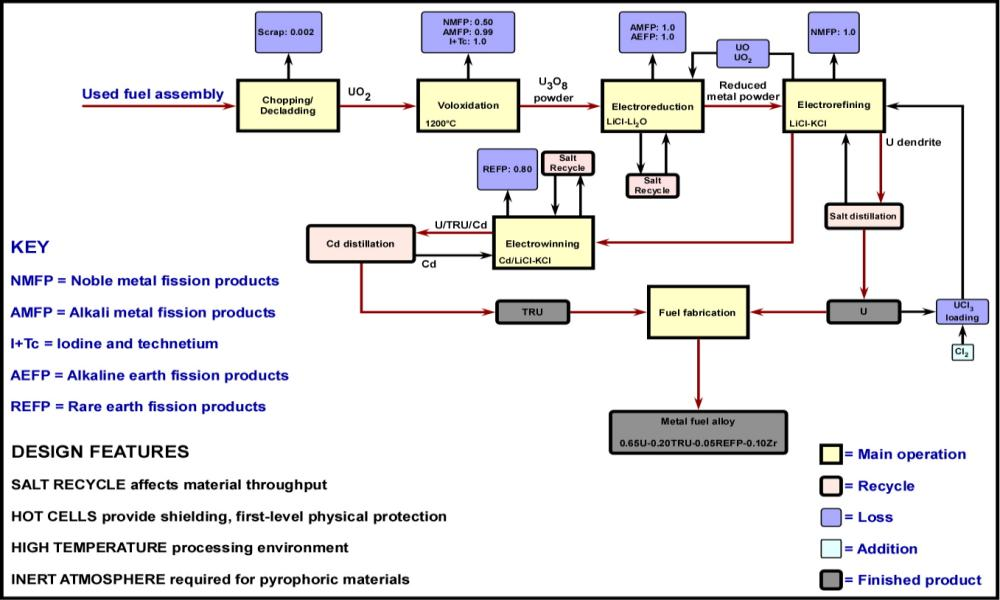
\includegraphics[width=0.80\textwidth]{pyroprocessing.flowsheet.jpg}
%        \caption{}
    \end{figure}
\end{frame}


\begin{frame}{}
    \begin{figure}
        \centering
        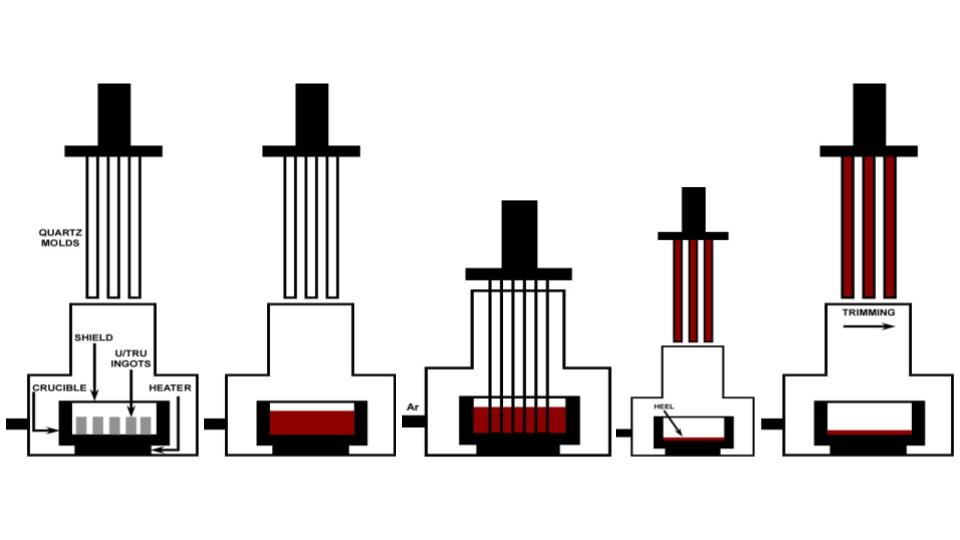
\includegraphics[width=0.80\textwidth]{fuel.fabrication.jpg}
%        \caption{}
    \end{figure}
\end{frame}


\begin{frame}{}
    \begin{figure}
        \centering
        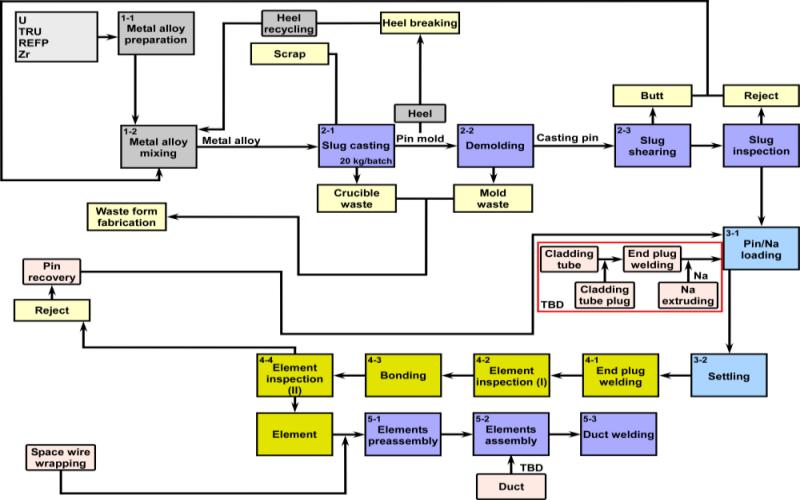
\includegraphics[width=0.80\textwidth]{fuel.fabrication.process.steps.jpg}
%        \caption{}
    \end{figure}
\end{frame}


\begin{frame}{Multiple failures, much more complexity}
    \begin{enumerate}[series=outerlist,topsep=0pt,itemsep=15pt,leftmargin=*,label=(\arabic*)]
        \item[]Getting material into the crucible
        \item[]Heater fails to sufficiently melt all the metal  
        \item[]Vacuum cannot be induced  
        \item[]Molds get stuck or break  
        \item[]Cannot remove heel  
        \item[]If one component fails the equipment fails
        \item[]Systems do not fail in the same way
    \end{enumerate}
\end{frame}


\begin{frame}[plain]{}
    \centering\LARGE\textbf{Data perception}
\end{frame}


\addtocounter{framenumber}{-1}
\begin{frame}{It is important to consider how to frame failure data or what the data actually is}
    \begin{enumerate}[series=outerlist,topsep=0pt,itemsep=11pt,leftmargin=*,label=(\arabic*)]
        \item[]Space shuttle program used as an example 8.1.9  
        \item[]At the time, failure rate was 1 in 25  
        \item[]2 catastrophic failures in 132 flights currently however
        \item[]Each shuttle operated for different number of missions with varying operating time (table 8.5)
        \item[]Total of 30946 operating hours = 4.5 operating years  
        \item[]1 failure in 15000 operating hours for 5 different shuttles  
        \item[]There is not any normalization in terms of failures per operating year
    \end{enumerate}
\end{frame}


\begin{frame}[plain]{}
    \centering\LARGE\textbf{Monte Carlo analysis}
\end{frame}


\addtocounter{framenumber}{-1}
\begin{frame}{Monte Carlo can be used to establish failure rates or \acs{mtf}}
    \begin{enumerate}[series=outerlist,topsep=0pt,itemsep=21pt,leftmargin=*,label=(\arabic*)]
        \item[]Monte Carlo simulation is very famous, but not fancy
        \item[]Generates values of a random variable based probability distributions
        \item[]Applied to wide variety of complex problems involving random behavior
    \end{enumerate}
\end{frame}


\begin{frame}{Monte Carlo can be used for \href{https://uidaho.pressbooks.pub/riskassessment/chapter/failure-rates-and-reliability/}{reliability}}
    \begin{equation}
        \LARGE
        R(T) = e^{-(\frac{T}{\eta})^{\beta}}
    \end{equation}

    \begin{enumerate}[series=outerlist,topsep=0pt,itemsep=3pt,leftmargin=*,label=(\arabic*)]
        \item[]$U \equiv R(T)$ -- U is a random number
    \end{enumerate}

    \begin{equation}
        \LARGE
        T = -\eta(ln \; U)^{\frac{1}{\beta}}
    \end{equation}

    \begin{enumerate}[series=outerlist,topsep=0pt,itemsep=3pt,leftmargin=*,label=(\arabic*)]
        \item[]When $\beta = 1$ we have the exponential distribution
    \end{enumerate}
\end{frame}


\begin{frame}{}
    \begin{figure}
        \centering
        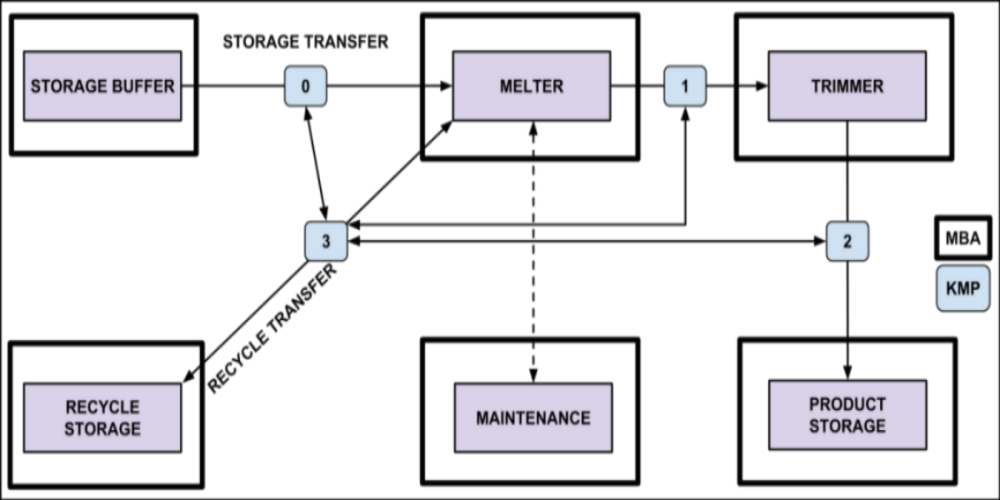
\includegraphics[width=0.80\textwidth]{des_fuel.fabrication.jpg}
%        \caption{}
    \end{figure}
\end{frame}


\begin{frame}{}
    \begin{figure}
        \centering
        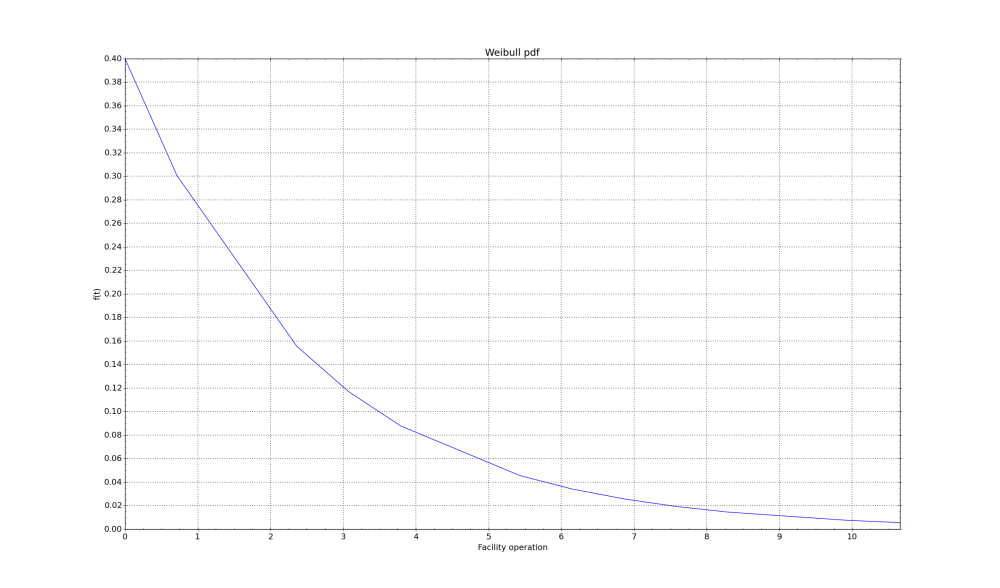
\includegraphics[width=0.89\textwidth]{img/weibull.jpg}
%        \caption{}
    \end{figure}
\end{frame}


\begin{frame}{}
    \begin{figure}
        \centering
        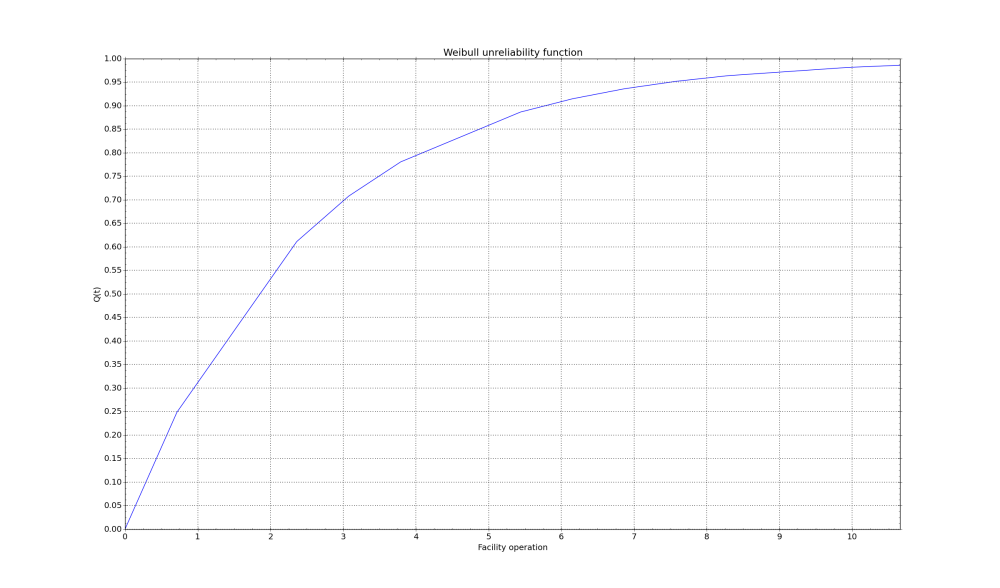
\includegraphics[width=0.90\textwidth]{unreliability.jpg}
%        \caption{}
    \end{figure}
\end{frame}


\begin{frame}{We can use the unreliability function to simulate failures}
    \begin{equation}
        \LARGE
        Q(t) = 1 - R(t)
    \end{equation}

    \begin{equation}
        \LARGE
        Q(t) = 1 - e^{-(\frac{t}{\eta})^{\beta}}
    \end{equation}

    \begin{enumerate}[series=outerlist,topsep=0pt,itemsep=15pt,leftmargin=*,label=(\arabic*)]
        \item[]Assume $\beta = 1$ for general failures
        \item[]$\lambda = 0.4$ per day
        \item[]Monte Carlo simulates area under the curve at t = T
        \item[]A 'hit' is an equipment failure
    \end{enumerate}
\end{frame}


\begin{frame}{}
    \texttt{campaign: 1\\
    operation time: 0.7144\\
    failure probability: 0.2486\\  
    failure test: 0.1808\\  
    failure}
    
    \vspace{0.10in}

    \texttt{campaign: 2\\
    operation time: 3.0762\\
    failure probability: 0.2486\\
    failure test: 0.6888\\
    no failure}

    \begin{enumerate}[series=outerlist,topsep=0pt,itemsep=5pt,leftmargin=*,label=(\arabic*)]
        \item[]New equipment is installed, so there is new distribution
        \item[]Early times the likelihood of failure is low 
        \item[]Later times it is higher because equipment is older
        \item[]\href{https://github.com/TheDoctorRAB/failure.testing}{Failure testing repository}
    \end{enumerate}
\end{frame}


\begin{frame}[plain]{}
    \centering\LARGE\textbf{Human error}
\end{frame}


\addtocounter{framenumber}{-1}
\begin{frame}{Human error probability is difficult to quantify}
    \begin{enumerate}[series=outerlist,topsep=0pt,itemsep=21pt,leftmargin=*,label=(\arabic*)]
        \item[]Because people generally behave stupidly even sober
        \item[]Or, different responses are elicited by people in the same environment
        \item[]What would be examples of human errors that could be quantified?
        \item[]Astronaut behavior in normal conditions and critical conditions
        \item[]Psychological stress
    \end{enumerate}
\end{frame}


\begin{frame}{Performance shaping factors account for human response to stressors}
    \begin{enumerate}[series=outerlist,topsep=0pt,itemsep=3pt,leftmargin=*,label=(\arabic*)]
        \item[]hot/cold  
        \item[]noise level   
        \item[]light level (my office is dark)  
        \item[]vibration  
        \item[]ergonomics
        \item[]experience and training
        \item[]management
        \item[]time
        \item[]stress
        \item[]equipment design/human machine interface
    \end{enumerate}
\end{frame}


\begin{frame}[plain]{}
    \centering\LARGE\textbf{Delphi technique}
\end{frame}


\addtocounter{framenumber}{-1}
\begin{frame}{The \href{https://uidaho.pressbooks.pub/riskassessment/chapter/failure-rates/}{Delphi technique}}
    \begin{enumerate}[series=outerlist,topsep=0pt,itemsep=21pt,leftmargin=*,label=(\arabic*)]
        \item[]Initially developed in the 1950s by Helmer and Dalkey at Rand Corp
        \item[]Controlled opinion feedback
        \item[]
            \begin{quote}
                \ldots to solicit expert opinion to the selection, from the point of view of a Soviet strategic planner, of an optimal U.S. industrial target system and to the estimation of the number of A-bombs required to reduce the munitions output by a prescribed amount.
            \end{quote}
    \end{enumerate}
\end{frame}


\begin{frame}{Delphi can be used to validate research outcomes}
    \begin{enumerate}[series=outerlist,topsep=0pt,itemsep=18pt,leftmargin=*,label=(\arabic*)]
        \item[]Impact analysis of changes to the international business environment
        \item[]Identify national park selection criteria
        \item[]Develop a taxonomy of organizational mechanisms
        \item[]Develop rules for a ceramic casting process
        \item[]Examine and explain how recruitment message specificity influences job seeker attraction to organizations
        \item[]Well suited to rigorously capture qualitative data or when knowledge is incomplete
    \end{enumerate}
\end{frame}


\begin{frame}{Assemble a panel of experts}
    \begin{enumerate}[series=outerlist,topsep=0pt,itemsep=1pt,leftmargin=*,label=(\arabic*)]
        \item[]\textbf{Mission}
        \item[]Build consensus with a panel
        \item[]Aircraft maintenance tasks - missing structural anomalies on an inspection (8.1.12)
        \item[]For composite structural material
            \vspace{0.05in}
        \item[]\textbf{Select panel and eliminate bias}
        \item[]Airline inspectors (regulations)  
        \item[]Structural experts from manufacturer(s)  
        \item[]Repair/mechanics experts
            \vspace{0.05in}
        \item[]\textbf{Calibrate the panel on the topic}
        \item[]Historical data on detecting cracks in the structure (not the same but close)  
        \item[]Inspection, procedures, etc.    
        \item[]In book example, estimated probabilities are presented
    \end{enumerate}
\end{frame}


\begin{frame}{Set problem boundaries and constraints}
    \begin{enumerate}[series=outerlist,topsep=0pt,itemsep=1pt,leftmargin=*,label=(\arabic*)]
        \item[]\textbf{Present the parameters of the task to evaluate}
        \item[]Qualitatively assess the problem  
        \item[]Discuss any direct historical experience from inspectors, mechanics  
        \item[]What kind of structural anomalies would be present?  
            \vspace{0.05in}
        \item[]\textbf{Perform the initial round of discussions on the error probability}
        \item[]Detecting anomalies 2" or less  
        \item[]Establish nominal probabilities for each class of crack 
            \vspace{0.15in}
        \item[]Discuss the results and iterate
            \vspace{0.15in}
        \item[]Repeat until consensus reached for each class
    \end{enumerate}
\end{frame}


\begin{frame}{Determine roadblocks}
    \begin{enumerate}[series=outerlist,topsep=0pt,itemsep=3pt,leftmargin=*,label=(\arabic*)]
        \item[]\textbf{Develop performance shaping factors}
        \item[]What factors would lower the probability of the task?  
        \item[]Lack of training; experience  
        \item[]Environmental conditions; lighting, etc.  
        \item[]Time to inspect
            \vspace{0.10in}
        \item[]\textbf{Establish the conditions where the task can be achieved satisfactorily}
            \vspace{0.10in}
        \item[]For use in human reliability analysis
    \end{enumerate}
\end{frame}


\begin{frame}[plain]{}
    \centering\LARGE\textbf{Event tree analysis}
\end{frame}


\addtocounter{framenumber}{-1}
\begin{frame}{An event tree is a graphical representation of a series of possible events in an accident sequence}
    \begin{enumerate}[series=outerlist,topsep=0pt,itemsep=17pt,leftmargin=*,label=(\arabic*)]
        \item[]Each event is either a fail or success with associated frequency
        \item[]Assumes events occur in sequence to a final state
        \item[]Event sequences follow from some initial event of interest, usually a component failure
        \item[]Downstream events follow from original event and subsequent events of other components
        \item[]Initiating event $\rightarrow$ event 1 $\rightarrow$ event N $\rightarrow$ Final State
        \item[]We covered ways to assess frequency - now we ask `What are the consequences?'
    \end{enumerate}
\end{frame}


\begin{frame}{Event trees apply forward logic}
    \begin{enumerate}[series=outerlist,topsep=0pt,itemsep=17pt,leftmargin=*,label=(\arabic*)]
        \item[]We start with the initiating events and work to what eventually happens
        \item[]Event trees are used to describe the major events in the accident sequence 
        \item[]Each event can then be further analyzed using a fault tree
        \item[]Event trees are accident sequence development tools
        \item[]We talked about WASH1400 that basically invented for nuclear power plants
        \item[]\href{http://www.nrc.gov/reading-rm/doc-collections/nuregs/staff/sr0492/}{\acs{nrc} handbook}
        \item[]Figure 12.3 in the book
    \end{enumerate}
\end{frame}


\begin{frame}{Event trees are essential to \acs{pra}}
    \begin{enumerate}[series=outerlist,topsep=0pt,itemsep=21pt,leftmargin=*,label=(\arabic*)]
        \item[]Visualize event chains following an accidental event
        \item[]Visualize barriers and sequence of activation
        \item[]Good basis for evaluating the need for new/improved procedures and safety functions
        \item[]Draws on prior \acsp{pra}, etc., to determine initiating events
        \item[]So it's a natural progression into \acs{pra} I,II,III
    \end{enumerate}
\end{frame}


\begin{frame}[plain]{}
    \centering\LARGE\textbf{Examples}
\end{frame}


\begin{frame}[plain]{}
    \centering\LARGE\textbf{Fire}
\end{frame}


\addtocounter{framenumber}{-2}
\begin{frame}{What events lead to \href{https://uidaho.pressbooks.pub/riskassessment/chapter/event-trees-2/}{fire?} -- Figure 12.2}
    \begin{figure}
        \centering
        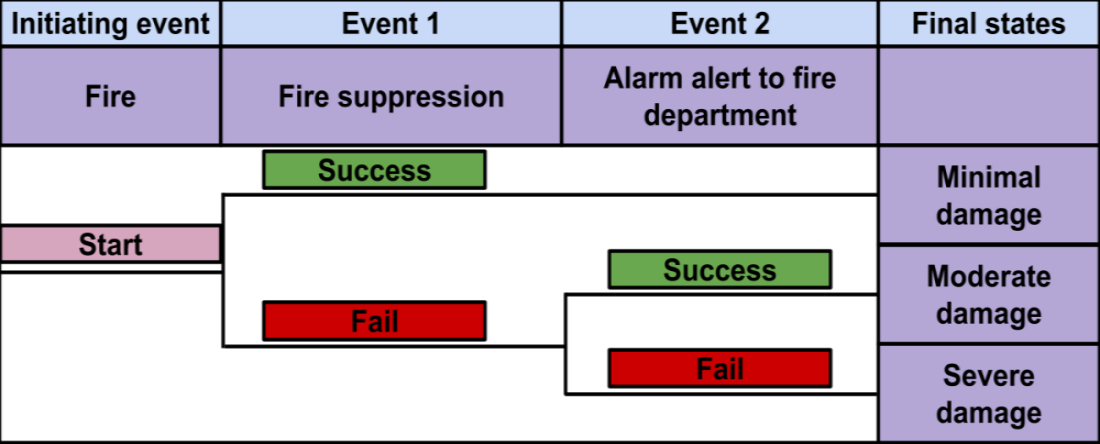
\includegraphics[width=0.90\textwidth]{event.tree_fire.jpg}
%        \caption{}
    \end{figure}
\end{frame}


\begin{frame}{Calculate probabilities and losses}
    \begin{figure}
        \centering
        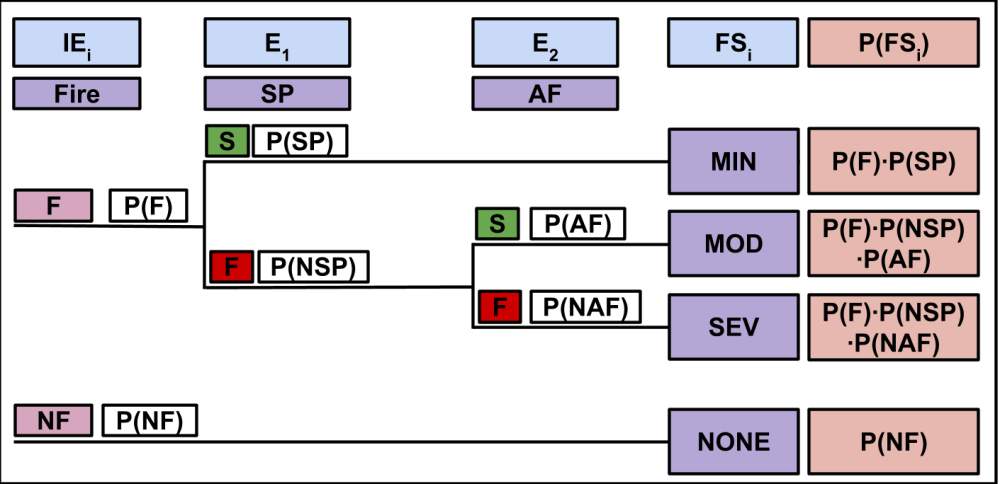
\includegraphics[width=0.90\textwidth]{event.tree_fire.loss.jpg}
%        \caption{}
    \end{figure}
\end{frame}


\begin{frame}[plain]{}
    \centering\LARGE\textbf{Pumps}
\end{frame}


\addtocounter{framenumber}{-1}
\begin{frame}{}
    \begin{figure}
        \centering
        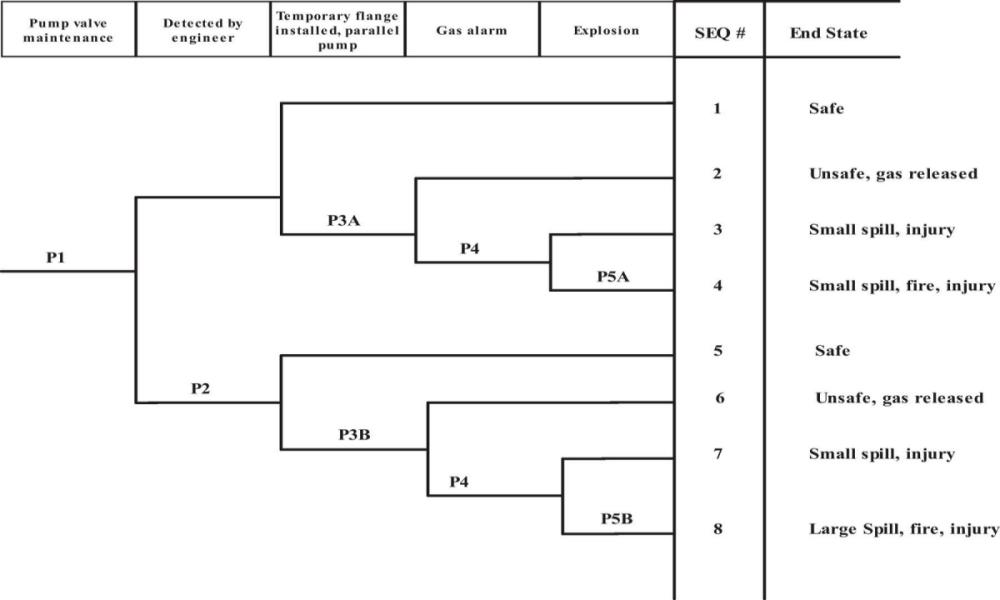
\includegraphics[width=0.90\textwidth]{event.tree_pump.valve.jpg}
%        \caption{}
    \end{figure}
\end{frame}


\begin{frame}[plain]{}
    \centering\LARGE\textbf{Fracking}
\end{frame}


\addtocounter{framenumber}{-1}
\begin{frame}{}
    \begin{figure}
        \centering
        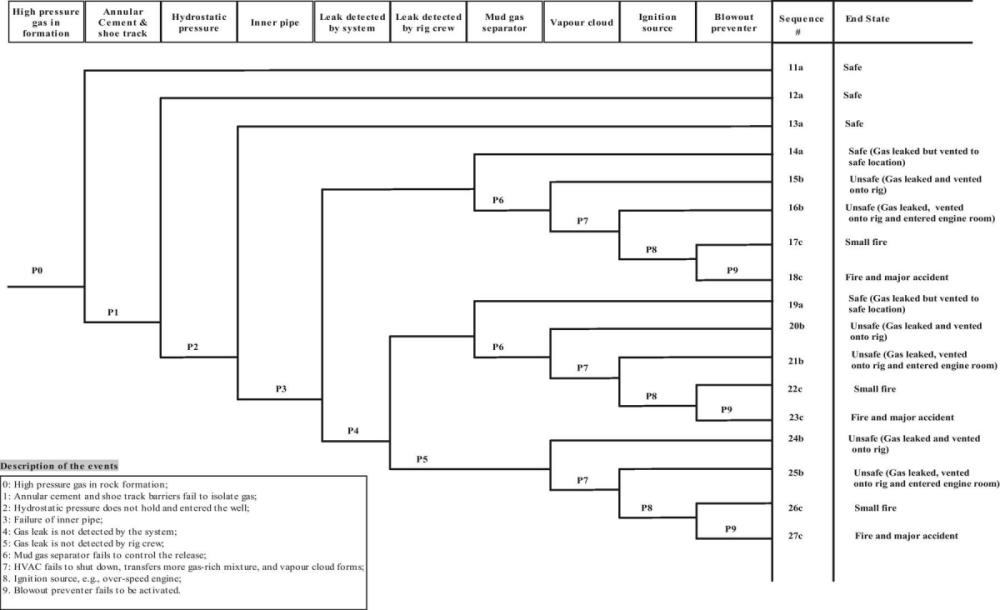
\includegraphics[width=0.80\textwidth]{event.tree_gas.jpg}
%        \caption{}
    \end{figure}
\end{frame}


\begin{frame}[plain]{}
    \centering\LARGE\textbf{\acs{loc}}
\end{frame}


\addtocounter{framenumber}{-1}
\begin{frame}{}
    \begin{figure}
        \centering
        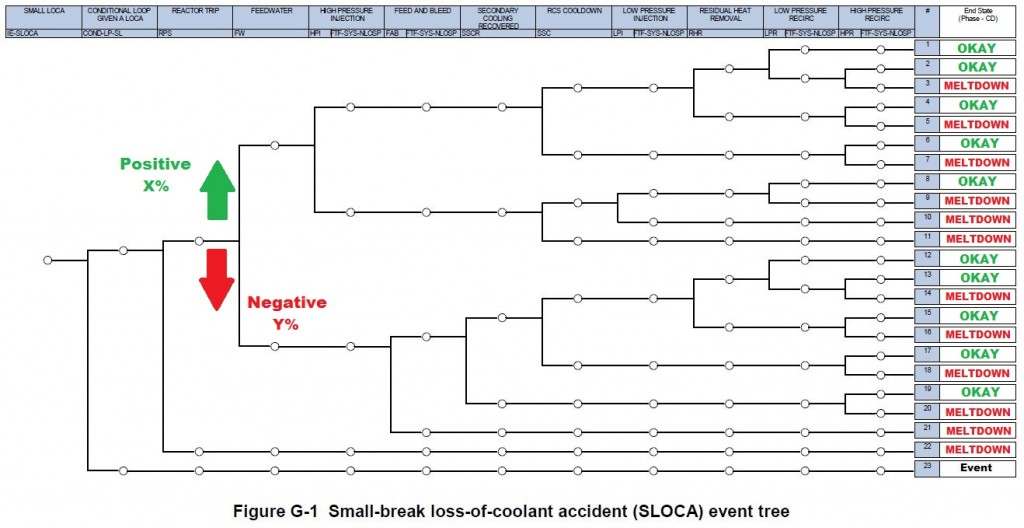
\includegraphics[width=0.95\textwidth]{event.tree_loca.jpg}
%        \caption{}
    \end{figure}
\end{frame}


\begin{frame}[plain]{}
    \centering\LARGE\textbf{Limitations}
\end{frame}


\addtocounter{framenumber}{-1}
\begin{frame}{But event trees have limitations}
    \begin{enumerate}[series=outerlist,topsep=0pt,itemsep=11pt,leftmargin=*,label=(\arabic*)]
        \item[]No standard for the graphical representation of the event tree
        \item[]Only one initiating event can be studied in each analysis
        \item[]Easy to overlook subtle system dependencies
        \item[]Not well suited for handling common cause failures (only independent events)
        \item[]Practical only when events can be ordered in time (chronology of events is stable) 
        \item[]Does not show acts of omission
        \item[]Difficult to represent interactions among events  
        \item[]Difficult to consider effects of multiple initiating events
        \item[]So we need other tools for comprehensive risk assessment
    \end{enumerate}
\end{frame}


\begin{frame}[plain]{}
    \centering\LARGE\textbf{Fault tree analysis}
\end{frame}


\addtocounter{framenumber}{-1}
\begin{frame}{Fault tree analysis is applied to identify areas to mitigate or prevent risk at all phases of system life cycle}
    \begin{enumerate}[series=outerlist,topsep=0pt,itemsep=13pt,leftmargin=*,label=(\arabic*)]
        \item[]Little things lead to catastrophic failures
        \item[]\href{https://www.faa.gov/lessons_learned/transport_airplane/accidents/JA8119}{Japan airlines}
        \item[]But before risk assessment was invented, most likely from common cause failures
        \item[]Advancements in technologies increased complexity and necessitated detailed safety analysis
        \item[]Developed by Bell Telephone Laboratories (1962) for Minuteman ICBM (can't find any information)
        \item[]Though it seems that not formalized as part of risk assessment until WASH1400
    \end{enumerate}
\end{frame}


\begin{frame}{Fault trees are a graphic to represent the interaction of failures and other events in a system}
    \begin{enumerate}[series=outerlist,topsep=0pt,itemsep=11pt,leftmargin=*,label=(\arabic*)]
        \item[]Top down, deductive failure analysis  
        \item[]Top event are hazards or failure modes (from event tree) -- \acs{loc}, emissions, explosions
        \item[]Decompose the top event using boolean logic (AND, OR)
        \item[]Bottom set of events are non-decomposable (basic events)
        \item[]Identify failures as a malfunction in a component requiring repair (pump shaft)
        \item[]Identify faults as malfunctions that self-repair once the governing condition is corrected (wet contacts for a switch; dry them)
        \item[]Undeveloped events are neglected due to low probability or effect on system
        \item[]\acs{fma} can be used as input
    \end{enumerate}
\end{frame}


\begin{frame}{Define the top event clearly and unambiguously}
    \begin{enumerate}[series=outerlist,topsep=0pt,itemsep=7pt,leftmargin=*,label=(\arabic*)]
        \item[]What is the event?  
        \item[]Where does the event occur?  
        \item[]When does the event occur?
        \item[]Immediate, necessary, and sufficient causes leading to the event
        \item[]Connect via logic gates (down)
        \item[]Get down to independent events  
        \item[]For which failure data is obtained (or distributions)  
        \item[]Work back up to compute top event probability
    \end{enumerate}
\end{frame}


\begin{frame}{Assemble a basic event matrix after defining the top event}
    \begin{enumerate}[series=outerlist,topsep=0pt,itemsep=21pt,leftmargin=*,label=(\arabic*)]
        \item[]Basic failure event -- description -- credible? (table 14.5)
        \item[]Assessing credibility = whether to include the event in the fault tree
        \item[]Coolant system flushing procedure in the car (14.7.1)
        \item[]Sprinkler system failure
        \item[]System design tool
    \end{enumerate}
\end{frame}


\begin{frame}[plain]{}
    \centering\LARGE\textbf{TAM airline}
\end{frame}


\addtocounter{framenumber}{-1}
\begin{frame}{\href{https://maps.app.goo.gl/nUTrfB5vhgz1zwSUA}{TAM Airlines Flight 3054} overran the runway and crashed into a warehouse (2007)}
    \begin{enumerate}[series=outerlist,topsep=0pt,itemsep=21pt,leftmargin=*,label=(\arabic*)]
        \item[]Use of fault trees for accident analysis with multiple failures (14.7.3)
        \item[]Airplane are an instructive example because we know a lot about them
        \item[]Warehouse next to gas station, which exploded
        \item[]199 fatalities
    \end{enumerate}
\end{frame}


\begin{frame}{What happened}
    \begin{enumerate}[series=outerlist,topsep=0pt,itemsep=21pt,leftmargin=*,label=(\arabic*)]
        \item[]Rain caused the runway to be wet
        \item[]Plane overran the runway
        \item[]Crossed the road(!)
    \end{enumerate}
\end{frame}


\begin{frame}{Background}
    \begin{enumerate}[series=outerlist,topsep=0pt,itemsep=17pt,leftmargin=*,label=(\arabic*)]
        \item[]20379 operating hours
        \item[]Jammed braking device reported the day before (thrust reverser)
        \item[]Landed and couldn't slow down
        \item[]Veered left and overshot runway over the major road
        \item[]Collided with warehouse
        \item[]Safety issues with insufficient length of the runway (faster speed, more distance to stop)
    \end{enumerate}
\end{frame}


\begin{frame}{Flight recorder}
    \begin{enumerate}[series=outerlist,topsep=0pt,itemsep=21pt,leftmargin=*,label=(\arabic*)]
        \item[]Thrusters in climb position just before touchdown
        \item[]Audio warning 2 seconds before touchdown for pilots to take manual control
        \item[]One idle, one at climb position at touchdown; both needed to be in idle position
        \item[](cause of veering left)
        \item[]So, what are some causes for this crash?
    \end{enumerate}
\end{frame}


\begin{frame}{}
    \begin{figure}
        \centering
        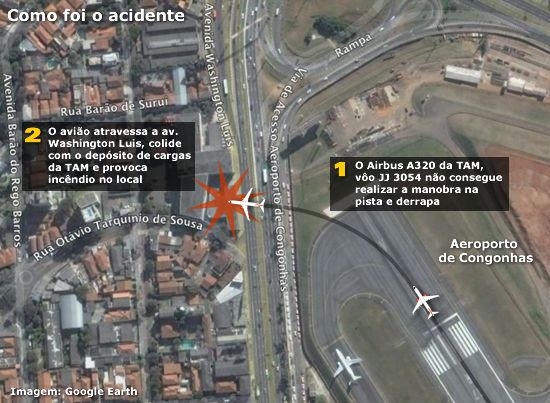
\includegraphics[width=0.80\textwidth]{brazil_airport.jpg}
%        \caption{}
    \end{figure}
\end{frame}


\begin{frame}{Top event is the airplane crash}
    \begin{enumerate}[series=outerlist,topsep=0pt,itemsep=11pt,leftmargin=*,label=(\arabic*)]
        \item[]Wet runway (hydroplaning, loss of vehicle control)  
        \item[]Rain
        \item[]Grooves cut in runway to drain and increase traction  
        \item[]Thrust reverser broken (known)
        \item[]Airline policy allowed aircraft to be flown with broken thrust reverser  
        \item[]Short runway   
        \item[]Airport policy allowed larger planes to land on runway  
        \item[]Experienced pilots had not had training in this situation  
    \end{enumerate}
\end{frame}


\begin{frame}[plain]{}
    \centering\LARGE\textbf{Building the fault tree}
\end{frame}


\addtocounter{framenumber}{-1}
\begin{frame}{How is the probability of crash calculated?}
    \begin{enumerate}[series=outerlist,topsep=0pt,itemsep=21pt,leftmargin=*,label=(\arabic*)]
        \item[]Gates aren't limited to only two events  
        \item[]Can be more than one level of intermediate causes
    \end{enumerate}
\end{frame}


\begin{frame}{}
    \begin{figure}
        \centering
        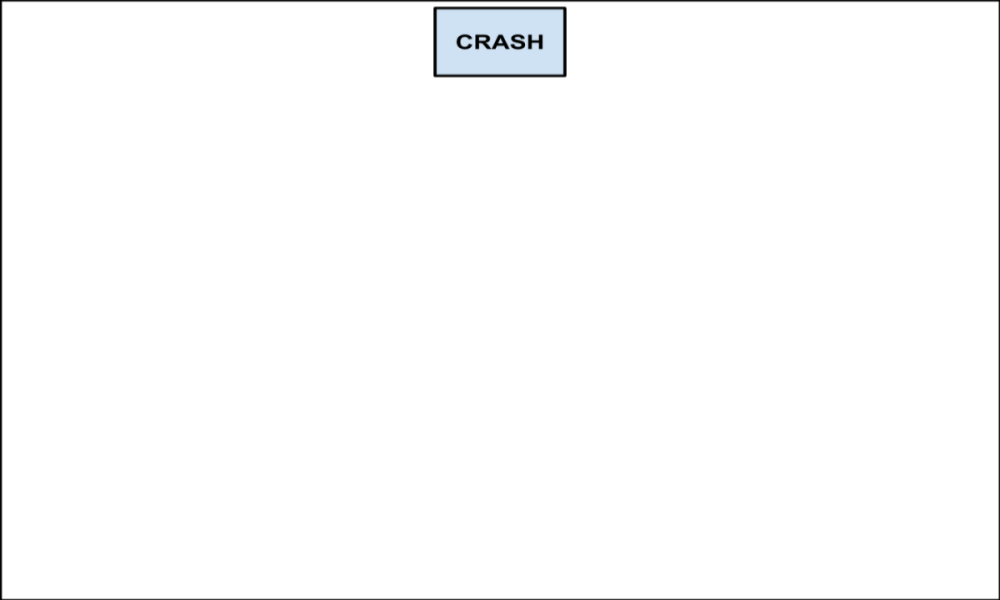
\includegraphics[width=0.80\textwidth]{fault.tree_plane.1.jpg}
%        \caption{}
    \end{figure}
\end{frame}


\begin{frame}{}
    \begin{figure}
        \centering
        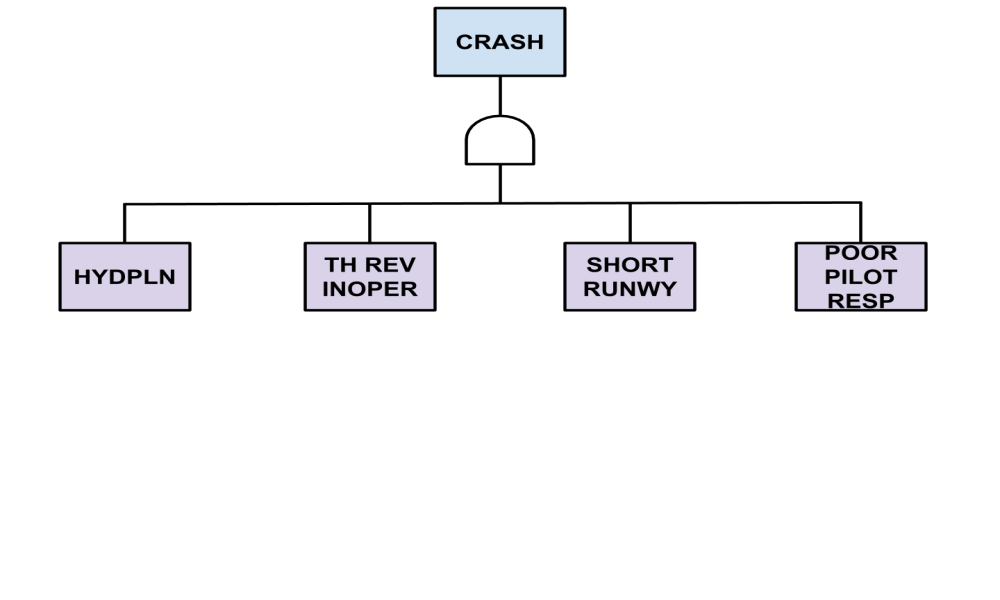
\includegraphics[width=0.80\textwidth]{fault.tree_plane.2.jpg}
%        \caption{}
    \end{figure}
\end{frame}


\begin{frame}{}
    \begin{figure}
        \centering
        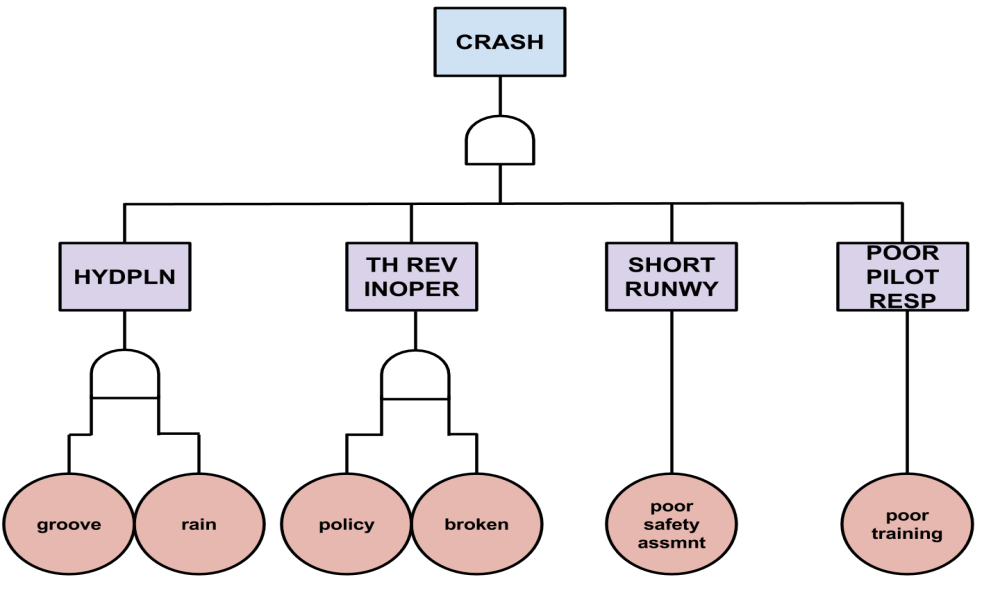
\includegraphics[width=0.80\textwidth]{fault.tree_plane.3.jpg}
%        \caption{}
    \end{figure}
\end{frame}


\begin{frame}[plain]{}
    \centering\LARGE\textbf{Doorbell}
\end{frame}


\addtocounter{framenumber}{-1}
\begin{frame}{}
    \begin{figure}
        \centering
        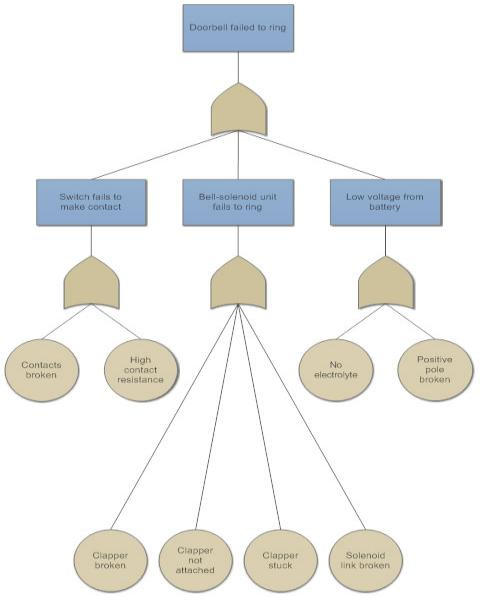
\includegraphics[width=0.45\textwidth]{fault.tree_doorbell.jpg}
%        \caption{}
    \end{figure}
\end{frame}


\begin{frame}[plain]{}
    \centering\LARGE\textbf{Lighting the room}
\end{frame}


\addtocounter{framenumber}{-1}
\begin{frame}{}
    \begin{figure}
        \centering
        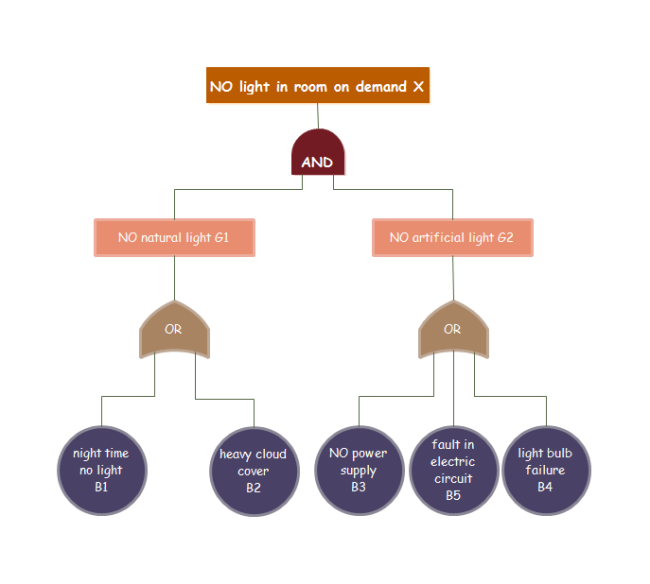
\includegraphics[width=0.65\textwidth]{fault.tree_room.jpg}
%        \caption{}
    \end{figure}
\end{frame}


\begin{frame}[plain]{}
    \centering\LARGE\textbf{Car crash}
\end{frame}


\addtocounter{framenumber}{-1}
\begin{frame}{}
    \begin{figure}
        \centering
        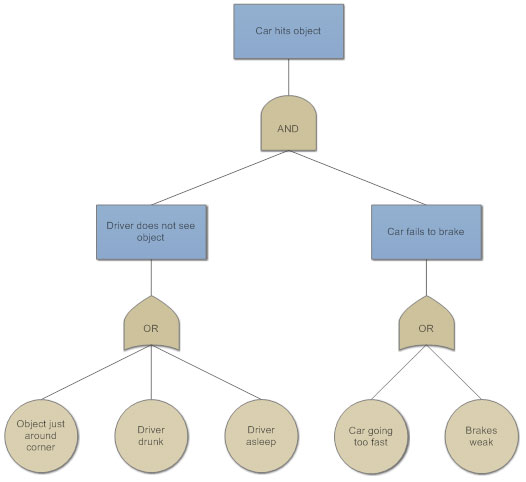
\includegraphics[width=0.55\textwidth]{fault.tree_car.jpg}
%        \caption{}
    \end{figure}
\end{frame}


\begin{frame}[plain]{}
    \centering\LARGE\textbf{Counterexample}
\end{frame}


\addtocounter{framenumber}{-1}
\begin{frame}{}
    \begin{figure}
        \centering
        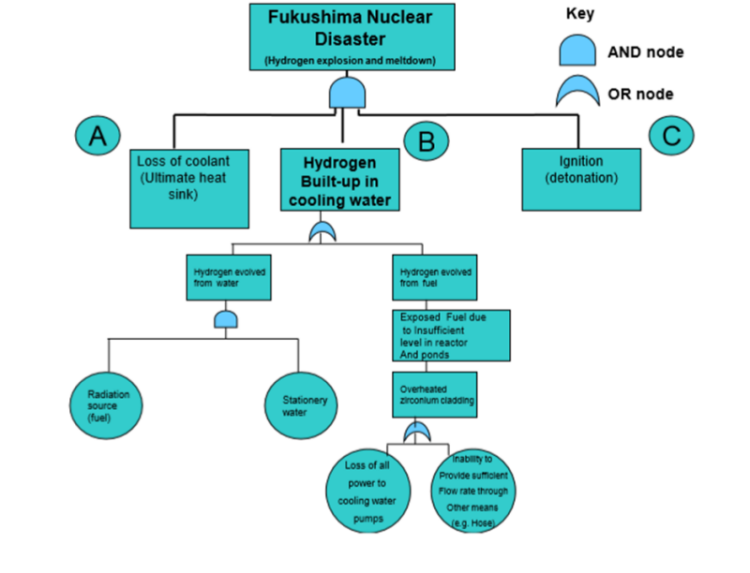
\includegraphics[width=0.80\textwidth]{fault.tree_fukushima.jpg}
%        \caption{}
    \end{figure}
\end{frame}


\begin{frame}[plain]{}
    \centering\LARGE\textbf{Limitations}
\end{frame}


\addtocounter{framenumber}{-1}
\begin{frame}{Of course, there are limitations}
    \begin{enumerate}[series=outerlist,topsep=0pt,itemsep=15pt,leftmargin=*,label=(\arabic*)]
        \item[]Undesirable events must be foreseen  
        \item[]We don't know what we don't know
        \item[]Each event analyzed singly
        \item[]Significant contributors to fault/failure must be anticipated or predicted
        \item[]Each initiator must be constrained to two conditional modes (AND/OR)
        \item[]Initiators at beneath a common gate must be independent 
        \item[]Still requires detailed knowledge of the system
    \end{enumerate}
\end{frame}


\begin{frame}[plain]{}
    \begin{figure}
        \centering
        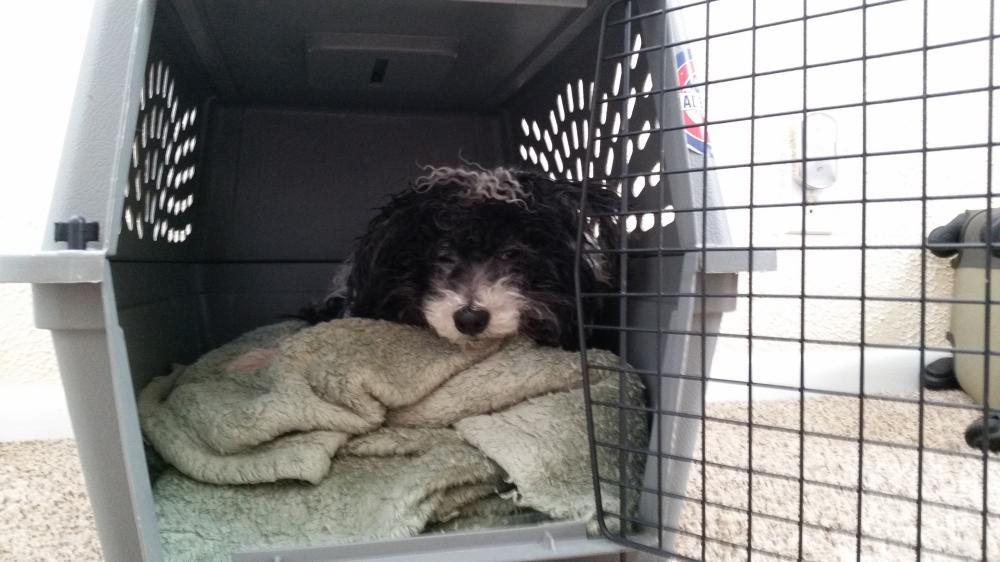
\includegraphics[width=0.85\textwidth]{final.jpg}
%        \caption{}
    \end{figure}
\end{frame}


%%%%%%%
%\begin{frame}{}
%    \begin{columns}
%
%        \begin{column}{0.50\textwidth}
%            \begin{enumerate}[series=outerlist,topsep=0pt,itemsep=21pt,leftmargin=*,label=(\arabic*)]
%                \item[]
%                \item[]
%            \end{enumerate}
%        \end{column}
%
%        \begin{column}{0.50\textwidth}
%            \begin{enumerate}[series=outerlist,topsep=0pt,itemsep=21pt,leftmargin=*,label=(\arabic*)]
%                \item[]
%                \item[]
%            \end{enumerate}
%        \end{column}
%
%    \end{columns}
%\end{frame}

%    \begin{figure}
%        \centering
%        \includegraphics[width=0.75\textwidth]{wsc.png}
%        \caption{\acs{wsc}}
%    \end{figure}


%\begin{frame}{References}
%    \bibliographystyle{nsf}
%    \footnotesize
%    \bibliography{references}
%\end{frame}
%%%%%%%


\end{document}
